\documentclass[a4paper,11pt]{article}
%\pdfoutput=1 % if your are submitting a pdflatex (i.e. if you have
%             % images in pdf, png or jpg format)

\usepackage{jcappub} % for details on the use of the package, please
                     % see the JCAP-author-manual
\usepackage{siunitx}
\usepackage[T1]{fontenc} % if needed


\title{\boldmath A title with some math: $x=1$}


%% %simple case: 2 authors, same institution
%% \author{A. Uthor}
%% \author{and A. Nother Author}
%% \affiliation{Institution,\\Address, Country}

\author{Jack Dinsmore}
\author{and Tracy Slatyer}
\affiliation{Massachusetts Institute of Technology \\Cambridge, MA, USA}

% e-mail addresses: one for each author, in the same order as the authors
\emailAdd{jtdinsmo@mit.edu}
\emailAdd{tslater@mit.edu}

\newcommand{\parens}[1]{\left(#1\right)}
\newcommand{\brackets}[1]{\left[#1\right]}
\newcommand{\expp}[1]{\exp \parens{#1}}
\newcommand{\fraci}[2]{#1 / #2}
\newcommand{\comment}[1]{\emph{\color{red}{#1}}}

\DeclareSIUnit\erg{erg}
\DeclareSIUnit\parsec{pc}



\abstract{Abstract...}



\begin{document}
\maketitle
\flushbottom



\section{Introduction}



\section{Methods \& Datasets}


\subsection{Observables}
To fit the luminosity functions described in section \ref{sec:lum-funcs}, we will use three observables: the total flux of the GCE $F_\text{GCE}$, the ratio of the total flux to the flux visible from point sources resolved by \textit{Fermi} $R_\text{r}$, and the number of resolved point sources $N_\text{r}$. We fix the first observable at $F_\text{GCE}= \SI{1.295e-09}{\erg\per\second}$ according to the methods outlined in section \ref{sec:total-lum}. We allow the other two observables to vary as functions of the parameters of the luminosity functions.

We will also discuss a third feature of a potential MSP population in the GC: the total number of MSPs $N_\text{GCE}$, resolved or unresolved. This number is not measurable, but serves as a useful reference to gauge the physicality of any population of MSPs. \comment{Mention that it's expected to be around 40,000.}


\subsection{Total GCE Luminosity}
\label{sec:total-lum}
Since an estimate of the total flux of the GCE is necessary for our data, we extract the total flux from several previous analyses of spectra using the following three methods and compare them. The spectral analyses we study here are refs. \cite{Zhong:2019ycb, Calore:2014xka, DiMauro:2021raz, Abazajian:2014fta, Gordon, Ajello}. Each reference reports the total flux $F_\gamma(E)$ observed in an energy bin centered on $E$. The spectra from these sources are reported in figure \ref{fig:all-spectra}
\begin{figure}
    \centering
    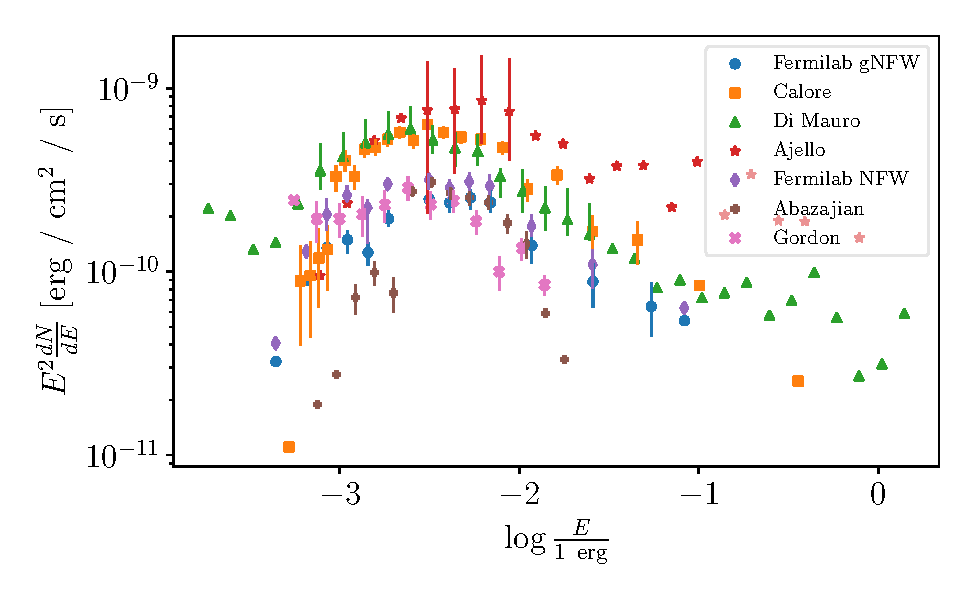
\includegraphics[width=0.5\textwidth]{figs/all-spectra.pdf}
    \caption{}
    \label{fig:all-spectra}
\end{figure}

\comment{Describe the sources: what's similar between them, what's different.}

We use compare three methods of extracting the total GCE flux from these analyses.
The first method is direct numerical integration of the spectra provided by each source. This method is most sensitive to the data measured by \textit{Fermi} and does not attempt to abstract over it with a smooth function.

However, numerical integration cannot account for the spectrum lying outside of \textit{Fermi}'s spectrum of sensitivity, and it may be oversensitive to experimental error. Therefore, we also consider a broken law fit to the data, of the same form as the NPTF luminosity function: eq. \ref{eqn:nptf}. It has four parameters: a constant of proportionality, the turnover flux $F_\text{b}$, and the slopes above and below the turnover flux $n_2$ and $n_1$. This function can then be analytically integrated over all flux values to get the total flux of the GCE. Many of the analyses cited above only report error bars on some points, because error bars on the other points are too large. We therefore fit only to the points with error bars reported. \comment{Mention the specific range fitted over}.

Unfortunately, for some analyses, the number of points reported with error bars is only slightly larger than the number of parameters of the broken power law function. To ensure that the fit result is less prone to statistical deviations of a small number of points, we use a third method in addition to the above two. Ref. \cite{Calore:2014xka} provides their fit parameters for their GCE flux spectral data: $F_\text{b} = $. $n_1 = -1.42$, $n_2 = 2.63$. \comment{Check for sign errors in the original. Also get the flux they provide.}. The third fitting method is to fix these three broken power law parameters at these values and allow only the overall normalization to vary.

An example of all three of these fitting methods applied to reference \cite{DiMauro:2021raz} is shown in figure \ref{fig:di-mauro-example}.
\begin{figure}
    \centering
    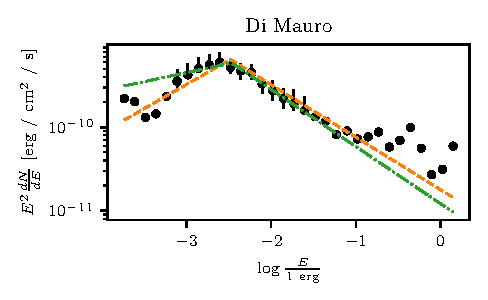
\includegraphics[width=0.5\textwidth]{figs/di-mauro-example.pdf}
    \caption{}
    \label{fig:di-mauro-example}
\end{figure}


In practice,
\begin{figure}
    \centering
    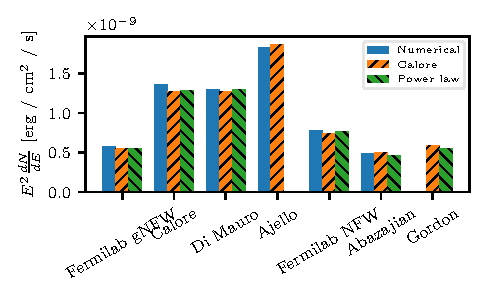
\includegraphics[width=0.5\textwidth]{figs/total-flux-bars.pdf}
    \caption{}
    \label{fig:total-flux-bars}
\end{figure}


\comment{Just double check that I normalized the power law correctly in parse\_spectrum.py.}


\subsection{GCE Spacial distribution}
\begin{equation}
    \rho_\text{NFW}(r) = \parens{\frac{r}{r_s}}^{-\gamma}\parens{1 + \frac{r}{r_s}}^{-3-\gamma}
    \label{eqn:nfw}
\end{equation}
where $\gamma = 1.2$ and $r_s = \SI{20}{\kilo\parsec}$ for this work.

\subsection{Luminosity Functions}
\label{sec:lum-funcs}
Previous work has interpreted this MSP model. Ref. \cite{Zhong:2019ycb} has proposed an exponentially damped power law luminosity function
\begin{equation}
    P_\text{Power law}(L) = L^{-\alpha} \expp{-\frac{L}{L_\text{max}}}\brackets{\Gamma\parens{1-\alpha, \frac{L_\text{min}}{L_\text{max}}}L_\text{max}^{1-\alpha}}^{-1}.
    \label{eqn:power-law}
\end{equation}
The function has been normalized so that $P_\text{Power law}(L)$ represents the probability that a given MSP has luminosity $L$. This luminosity function restricts the range of luminosities to $[L_\text{min}, \infty)$, where $L_\text{min}$, $L_\text{max}$, and $\alpha$ are free parameters. \comment{The following should probably be moved to the introduction, where Fermilab's research is described.} This reference found that $(\SI{1e29}{\erg\per\second}, \SI{1e35}{\erg\per\second}, 1.94)$ is required reproduced observations. They find that this model admits three million MSPs in the GCE, which differs from estimates based on the physical properties of observed MSPs that estimate the number of MSPs at the Galactic center at the order of 40,000 \cite{citation_needed}.

Ref. \cite{osti_1305131} proposes a power law luminosity function of
\begin{equation}
    P_\text{Log normal}(L)= \frac{\log_{10} e}{\sigma \sqrt{2\pi} L}\expp{-\frac{\parens{\log_{10} L - \log_{10} L_0}^2}{2\sigma^2}},
    \label{eqn:log-normal}
\end{equation}
where $L_0$ and $\sigma$ are free parameters. The ref. fits this model to data from globular cluster (GCL) data, yielding values $L_0 = \SI{8.8e33}{\erg\per\second}$ and $\sigma=0.62$. It predicts thousands of MSPs to occupy the GCE if the entire excess is to be explained by MSPs.

Ref. \cite{Ploeg:2020jeh} proposes several more intricate luminosity functions, derived from a model of the pulsars themselves. They find that the same model may be used for resolved, globular cluster MSPs in the Galactic disk and unresolved MSPs at the Galactic center. We use their luminosity function generated for the galactic disk. It closely resembles a log normal luminosity function as in equation \ref{eqn:log-normal}, where $L_0 = \SI{1.61e+32}{\erg\per\second}$ and $\sigma=0.700$.

Finally, ref. \cite{Lee:2015fea} proposes a broken-power law luminosity function of
\begin{equation}
    P_\text{NPTF}(L) = \parens{\frac{\parens{1-n_1}\parens{1-n_2}}{L_b \parens{n_1 - n_2}}}\begin{cases}
        \parens{\fraci{L}{L_\text{b}}}^{-n_{1}} & L < L_{b} \\
        \parens{\fraci{L}{L_\text{b}}}^{-n_{2}} & L > L_b
    \end{cases}
    \label{eqn:nptf}
\end{equation}
where the free parameters  $n_1$, $n_2$, and $L_b$ were found via a Non-Poissonian Template Fitting model (NPTF) to be $(18.2, -0.66, \SI{8.66e+33}{\erg\per\second})$ for an NFW-squared-distributed population of MSPs named NFW PS. The pxxxaper proposes a second luminosity function named Disk PS with parameters $(17.5, 1.4, \SI{3.34e+35}{\erg\per\second})$, which is unnormalizable except when a minimum luminosity of pulsars $L_\text{min}$ is introduced. We set $L_\text{min}=\SI{1e29}{\erg\per\second}$, which is the same minimum pulsar luminosity used by ref. \cite{Zhong:2019ycb}. The turnover luminosity $L_\text{b}$ was given as a photon flux value in units of photons per centimeter squared per second; the process used to convert from photon flux to luminosity is detailed in the methods section.

All the above-mentioned luminosity functions are shown in figure \ref{fig:lum-funcs}.

\begin{figure}
    \centering
    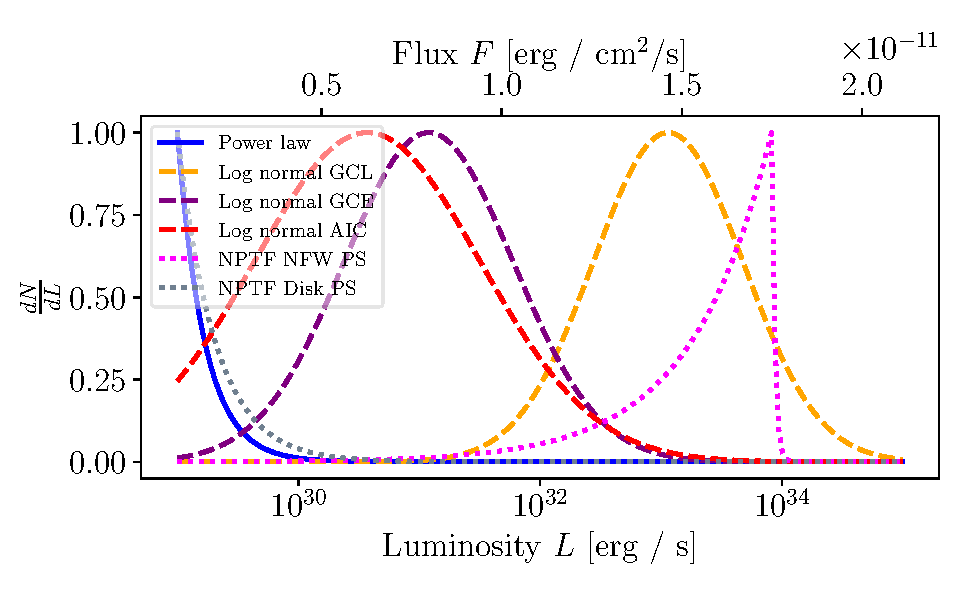
\includegraphics[width=0.49\textwidth]{figs/lum-funcs.pdf}
    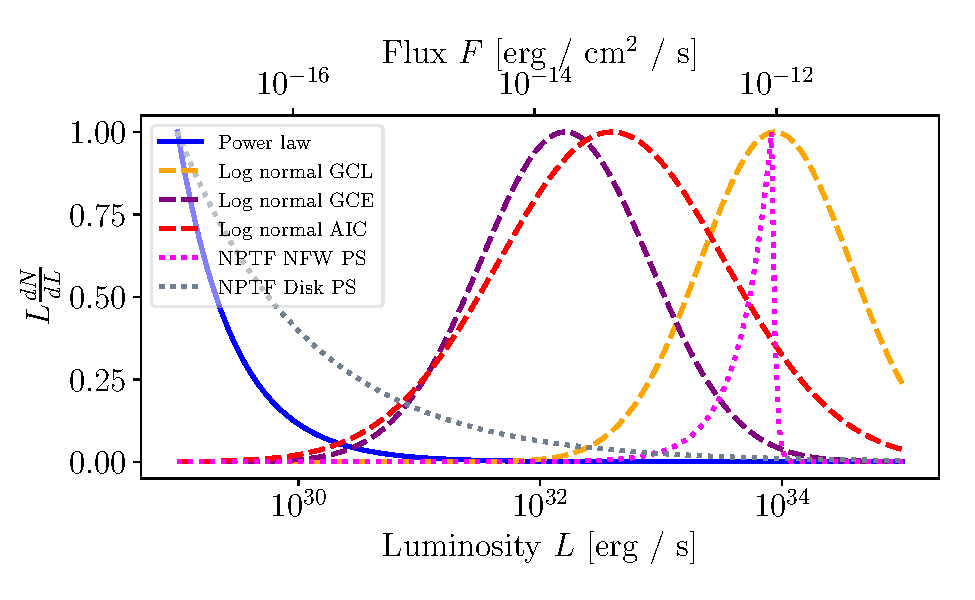
\includegraphics[width=0.49\textwidth]{figs/l-lum-funcs.pdf}
    \caption{\textit{Left:} Power law, GCL log normal, GCE log normal, and NPTF luminosity functions for MSPs in the GCE, vertically rescaled. \textit{Right:} Same plot as \textit{left} but weighted by luminosity.}
    \label{fig:lum-funcs}
\end{figure}


\subsection{Sensitivity Models}
The \textit{Fermi} telescope does not detect every pulsar in the GC; background emission obscures dimmer pulsars, and statistical effects cause some bright sources to be unresolved. We make use of three sensitivity models to model these factors.

The first, and simplest, is a step function luminosity model. It asserts that all point sources with $L>L_\text{th}$ are resolved, and none with $L<L_{\text{th}}$. Here, $L_\text{th} = \SI{e34}{\erg\per\second}$. This sensitivity model is the one used by ref. \cite{Zhong:2019ycb} to obtain the parameters of the power law luminosity function described in the paragraph after eq. \ref{eqn:power-law}. The four properties we intend to measure are then given by
\begin{equation}
    \begin{split}
        L_\text{GCE} &= N_\text{GCE}\int_{L_\text{min}}^\infty L P(L) dL \,, \qquad
        L_\text{r} = N_\text{GCE}\int_{L_\text{th}}^\infty L P(L) dL \,, \\
        N_\text{r} &= N_\text{GCE}\int_{L_\text{th}}^\infty P(L) dL \,,
        \label{eqn:observables-sens-1}
    \end{split}
\end{equation}
where $N_\text{GCE}$ is a normalization constant, fixed by requiring that $L_\text{GCE}$ reproduces the flux $F_\text{GCE}$ observed. The conversion between $L_\text{GCE}$ and $F_\text{GCE}$ is outlined in appendix \ref{app:lum-to-flux}.

The second sensitivity model acknowledges the effect of background flux on resolvability and uses a position-dependent flux threshold $F_\text{th}(b, l)$ published by the \textit{Fermi} team \cite{Fermi-LAT:2019yla, Ballet:2020hze} (figure \ref{fig:sensitivity}). \comment{Here, I could talk about how to convert between flux and luminosity and then use the mean of this map to assess how accurate 1e34 ergs/s actually is.}. To calculate the four properties of GC MSP populations, we use
\begin{equation}
    \begin{split}
        F_\text{GCE} &= \int_\Omega d\Omega \int_0^\infty s^2 ds A \rho_{NFW}^2(r)\int_{L_\text{min}}^\infty dL \frac{L}{4\pi s^2}P(L)\,, \\
        N_\text{GCE} &= \int_\Omega d\Omega \int_0^\infty s^2 ds A \rho_{NFW}^2(r)\,, \\
        F_\text{r} &= \int_\Omega d\Omega \int_0^\infty s^2 ds A \rho_{NFW}^2(r)\int_{4\pi s^2F_\text{th}(b,\ell)}^\infty dL \frac{L}{4\pi s^2}P(L)\,, \\
        N_\text{r} &= \int_\Omega d\Omega \int_0^\infty s^2 ds A \rho_{NFW}^2(r)\int_{4\pi s^2F_\text{th}(b,\ell)}^\infty dL P(L) \,. \\
        \label{eqn:observables-sens-2}
    \end{split}
\end{equation}
Here, $\Omega$ represents the $20^\circ \times 20^\circ$ region of interest with $|b| < 2^\circ$ cut out, and $A$ is the coefficient of equation \ref{eqn:nfw}, fixed by forcing $F_\text{GCE}$ to equal the observed value. In equation \ref{eqn:observables-sens-2} represents the distance to the galactic center from the point of integration, and is determined by the law of cosines:
$r^2 = s^2 + r_c^2 - 2r_c s \cos \ell$.

\begin{figure}
    \centering
    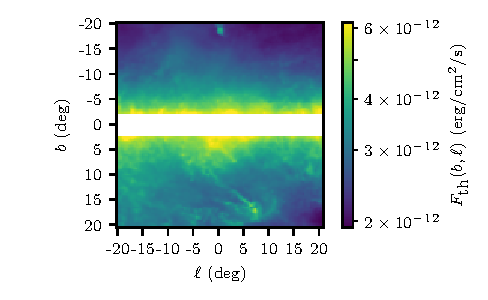
\includegraphics[width=0.7\textwidth]{figs/sensitivity-map.pdf}
    \caption{Position-dependent flux thresholds required to resolve an MSP, published by refs. \cite{Fermi-LAT:2019yla, Ballet:2020hze}.}
    \label{fig:sensitivity}
\end{figure}

The third and final sensitivity model takes into account the statistical fluctuation of photons from point sources. Ref. \cite{Ploeg:2020jeh} models the probability that a point source with average flux $F$ is resolved as
\begin{equation}
    P_\text{r}(F) = \frac{1}{\sigma_\text{th} F\sqrt{2\pi}} \expp{-\frac{(\ln F - (F_\text{th}(\ell, b) - K_\text{th}))^2}{2\sigma_\text{th}^2}}
    \label{eqn:ploeg-smoothing}
\end{equation}
where $K_\text{th}$ and $\sigma_\text{th}$ were determined via an MCMC fit to globular cluster MSPs. \comment{What are the values?} The observables are calculated simply by multiplying the integrand of the luminosity integral in equation \ref{eqn:observables-sens-2} by $P_r(L/4\pi s^2)$ for $F_\text{r}$ and $N_\text{r}$. (Not for $F_\text{GCE}$, because we do not require that the $F_\text{GCE}$ flux be resolved.)






\section{Results}



\section{Future Sensitivity}



\section{Conclusion}



\appendix
\section{Conversion Between GCE Luminosity and Flux}
\label{app:lum-to-flux}
\comment{Copy most of this from the January summary, if I include it.}





\acknowledgments

This is the most common positions for acknowledgments. A macro is
available to maintain the same layout and spelling of the heading.

\paragraph{Note added.} This is also a good position for notes added
after the paper has been written.





% The bibliography will probably be heavily edited during typesetting.
% We'll parse it and, using the arxiv number or the journal data, will
% query inspire, trying to verify the data (this will probalby spot
% eventual typos) and retrive the document DOI and eventual errata.
% We however suggest to always provide author, title and journal data:
% in short all the informations that clearly identify a document.


\bibliographystyle{plain}
\bibliography{gce.bib}

\end{document}
